\documentclass{lug}
\usepackage{graphicx}
\usepackage{amsmath}
\usepackage{bm}
\usepackage{color}

\title{My Beamer Template}
\author{Some Authors, et. al}
\institute{\textbf{Presented By:} \\ A Student \\ Department of Computer Science\\Colorado School of Mines}
\date{\today}

\begin{document}

\section{Motivation}
\frame{
    \frametitle{What's the Motivation?}
    Math is easier $$\sum_1^X \sum_1^Y \sum_1^Z xyz$$
    Making slides is fun!
}

\frame{
    \frametitle{Some Examples}
    \begin{itemize}[<+->]
        \item Beamer is fun!
        \item Beamer can be faster than PowerPoint! 
        \item You can edit using VIM! Or Overleaf if you like... 
    \end{itemize}
    \textbf{Goal}: Learning Beamer to make great looking presentations!
}

\section{Approach}
\frame{
    \frametitle{What is the Approach?}
    \begin{center}
        Beamer is as intuitive as gradient descent!\\
        $$\theta_{t+1} = \theta_t - \alpha_t \nabla f(\theta_t)$$
        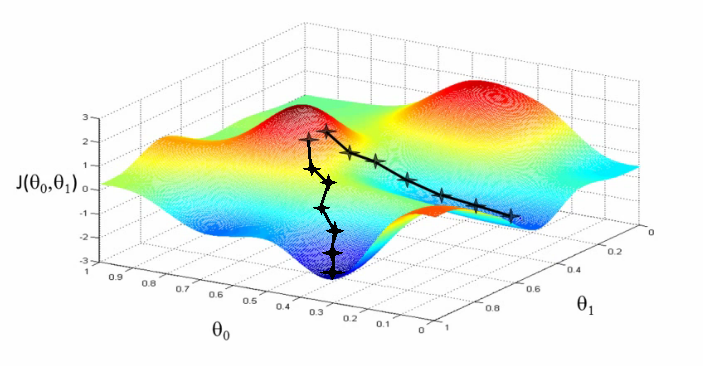
\includegraphics[scale=.6]{images/gradient_descent.png}
    \end{center}
}

\section{Experiments}
\frame{
    \frametitle{Some Cool Experiments}
    \begin{itemize}[<+->]
        \item Once you get the hang of it you'll never go back!
        \item Try `vimtutor' on the command line if you want a break!
    \end{itemize}
}

\frame{
    \begin{center}
        \Huge{Questions/Discussion}\\
    \end{center}
}

\nocite{*} % Include everything in the .bib file.
\bibliographystyle{plainnat}
\bibliography{beamer-template}

% that's all, folks
\end{document}
